% vim:syntax=tex
requirements. Feature location techniques have been a favored activity in

In this section we provide an overview of the document extraction and retreival process
used for feature location.
We also provide an overview of two topic models,
latent semantic indexing (LSI) and latent Dirichlet allocation (LDA),
and review closely related work.

\subsection{Document Extraction and Retrieval Process}


\begin{figure*}
\vspace{2mm}
\centerline{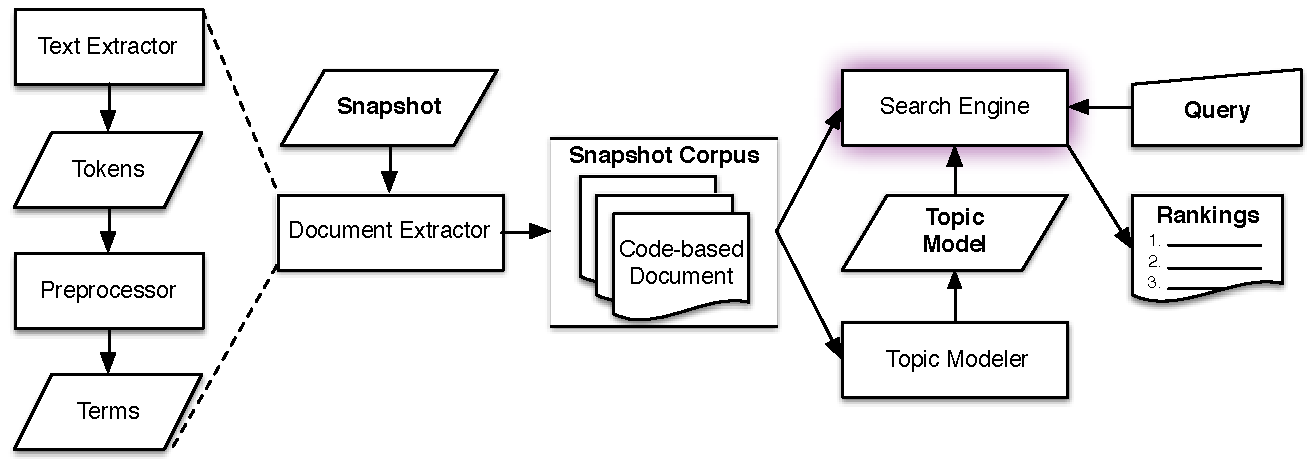
\includegraphics[width=.75\textwidth]{figures/snapshot-flt}}
\caption{Feature location using snapshots}
\label{fig:snapshot}
\vspace{-2mm}
\end{figure*}

We use the following terminology to describe document extraction of source code.
A \textit{word} is the basic unit of discrete data in a software lexicon and is a sequence of letters.
A \textit{token} is a sequence of non-whitespace characters containing one or more words.
An \textit{entity} is a named source element such as a method,
and an \textit{identifier} is a token representing the name of an entity.
\textit{Comments} and \textit{literals} are sequences of tokens delimited by language-specific markers (e.g., /* */ and quotes).
The \textit{document} which corresponds to a class is a sequence of words $d = (w_1, \ldots, w_m)$,
and a \textit{corpus} is a set of documents (i.e., classes) $D = (d_1, \ldots, d_n)$.

The left side of Figure~\ref{fig:snapshot} illustrates the document extraction process.
A document extractor takes source code as input and produces a corpus as output.
Each document in the corpus contains the words associated with a class.
The text extractor is the first part of the document extractor.
It parses the source code and produces a token stream for each class.
The preprocessor is the second part of the document extractor.
It applies a series of transformations to each token and
produces one or more words from the token.
The transformations~\cite{Marcus-etal:2004,Marcus-Menzies:2010}: % that we use are:
\begin{itemize}
    \item {\it Splitting}: separate tokens into constituent words
        based on common coding style conventions (e.g., the use of camel case or underscores)
        and on the presence of non-letters (e.g., punctuation or digits)
    \item {\it Normalizing}: replace each upper case letter with the corresponding
        lower case letter
    \item {\it Filtering}: remove common words such as articles (e.g., `an' or `the'),
        programming language keywords, standard library entity names, or short words
\end{itemize}

The right side of Figure~\ref{fig:snapshot} illustrates the retrieval process.
The main step of the retrieval process is to build the search engine.
The search engine is constructed from the topic model trained from the corpus.
The primary function of the search engine is to rank documents in relation to the query.
The search engine performs a pairwise classification of the query
to each document and ranks the documents according score.

To accomplish the classification step using a topic model,
the search engine infers $\theta_{Snapshot}$, i.e.,
the topic-document probability distribution of each document in the snapshot corpus,
as well as $\theta_{Query}$, i.e., the topic-document probability distribution  of the query.
Then a similarity measure for probability distributions, such as 
cosine similarity or Hellinger distance, can be used to make pairwise comparisons
between $\theta_{Query}$ and $\theta_{Snapshot}$.
Hellinger distance ($H$) can be defined as:

\begin{equation}
    H(P, Q) = \frac{1}{\sqrt{2}} \; \sqrt{\sum_{i=1}^{k} (\sqrt{P_i} - \sqrt{Q_i})^2}
\end{equation}

where $P$ and $Q$ are for two discrete probability distributions of length $k$.

\begin{comment}
\begin{equation}
    H(P, Q) = \frac{1}{\sqrt{2}} \; \bigl\|\sqrt{P} - \sqrt{Q} \bigr\|_2
\end{equation}
\end{comment}



\subsection{Latent Semantic Indexing}

Latent semantic indexing~\cite{Deerwester-etal:1990} is an indexing and
retrieval methodology. LSI uses a statistical technique, singular value
decomposition to identify patterns within the unstructured data, identifying
relationships between terms and documents, placing documents that are related
close to one another creating a semantic space. That is, LSI estimates the
latent structure by taking each document in the corpus and forming weighted
vectors applying cosine similarity to the vectors measuring the semantic
similarities between documents~\cite{Binkley-Lawrie:2010}.

\subsection{Latent Dirichlet Allocation}

Latent Dirichlet allocation~\cite{Blei-etal:2003} is a generative topic model.
LDA models each document in a corpus of discrete data as a finite mixture over
a set of topics and models each topic as an infinite mixture over a set of
topic probabilities.  That is, LDA models each document as a probability
distribution indicating the likelihood that it expresses each topic and models
each topic that it infers as a probability distribution indicating the
likelihood of a word from the corpus being assigned to the topic.


\subsection{Feature Location} 

A feature \cite{Biggerstaff} is a visible functionality within the source code
(feature is defined weakly throughout the literature because of the vast
context in which it can be used). Feature (or concept) location is a program
comprehension technique to locate specific source code elements (i.e., methods)
within the source code that relate to specific functional
requirements~\cite{972777, biggers2014configuring}. Locating functionalities
within the source code is a prerequisite for software evolution, or incremental
change.  Identifying features is a specifically crucial and frequent task for
developers, when adding new features, modifying existing features and removing
unwanted features (e.g.  bugs)~\cite{1309648, dit2013feature}. Locating bugs,
or bug localization~\cite{4656405} is analogous to removing unwanted features.    

Feature location is commonly categorized as a static, dynamic or a hybrid
technique involving a combination of the two. Static feature
location~\cite{biggers2014configuring} is a method that statistically analyzes
static documents, or source code. This is done by manually or automatically
analyzing the text to explore the dependencies within the structure. Dynamic
feature location applies a statistical analysis to the execution trace of a
specific scenario, therefore requiring a working system.~\cite{972777,4181710}
Hybrid techniques~\cite{1183929} involve a combination of a static analysis of
the source text and an analysis of scenarios in the execution trace. By
blending the two it was found that this technique was applicable to working
systems in providing higher precision for locating features.~\cite{4181710,
ernst2004static, revelleimproving} In this study, we are applying two static techniques, an LDA based FLT and an LSI based FLT. 

We now review research focusing on each of these techniques 


